\part{Soft Theorem}
% 计数器清零,每个part都要引用,除了part1
\setcounter{theorem}{0}
\setcounter{definition}{0}
\setcounter{lemma}{0}
\setcounter{sidenote}{1}
\section{Review on the quantization of gravity}
本节采用\cite{Badger:2023eqz}中的记号简要回顾引力量子化以及树图顶点项。众所周知微扰量子引力是不可重整化的,所以只能看作是一个有效理论,但好就好在它的低能极限是可以用于计算引力波振幅的\cite{Goldberger:2004jt,Bern:2019crd,Mogull:2020sak}。

取自由引力场拉式量为:
\begin{equation}
	\mathcal{L}_{EH}=\frac{2}{\kappa^2}\sqrt{-g}R,\quad \kappa=\sqrt{32\pi G}
\end{equation}
然后在平直度规附近做微扰:
\begin{equation}
	g_{\mu\nu}=\eta_{\mu\nu}+\kappa h_{\mu\nu}
\end{equation}
代入到$\mathcal{L}_{EH}$进行计算得到:
\begin{equation}
	\begin{aligned}
		\mathcal{L}_{\mathrm{EH}}& =\partial_{\alpha}h\partial_{\beta}h^{\alpha\beta}-\partial_{\alpha}h_{\beta\gamma}\partial^{\beta}h^{\alpha\gamma}-\frac{1}{2}(\partial_{\alpha}h)^{2}+\frac{1}{2}(\partial_{\gamma}h_{\alpha\beta})^{2}  \\
		&+\text{total derivatives}+\mathcal{O}\left(\kappa,h^{3}\right).
	\end{aligned}
\end{equation}
其中$h\equiv h^\alpha_\alpha$。这一堆都是$(\partial h)^2$项,对应动能项,显然由于没有$h^2$项,所以引力子质量为0。后面的高阶项意味着引力子之间是有自相互作用的。

由于广义相对论是微分同胚不变的,所以他其实也是个规范理论,不同的坐标系就意味着不同的规范,度规分量的变换正对应于场的规范变换。那么我们对$h_{\mu\nu}$进行路径积分时就必须在规范下进行,这可以使用F-P鬼场方法来系统的处理。比较常用的规范选取是下面的de-Donder规范:
\begin{equation}
	G_\mu\equiv\partial^\nu h_{\mu\nu}\frac{1}{2}\partial_\mu h=0
\end{equation}
这导致规范固定项:
\begin{equation}
	{\mathcal L}_{\mathrm{GF}}=G_{\mu}G^{\mu}=\partial^{\nu}h_{\mu\nu}\partial^{\rho}h^{\mu}{}_{\rho}+\frac{1}{4}(\partial_{\mu}h)^{2}-\partial^{\nu}h_{\mu\nu}\partial^{\mu}h
\end{equation}
以及鬼场:
\begin{equation}
	\mathcal{L}_{\mathrm{GH}}=-\bar{b}^{\mu}\left(\kappa\frac{\delta G_{\mu}}{\delta\xi^{\nu}}\right)b^{\nu}
\end{equation}
de-Donder规范下:
\begin{equation}
	\kappa\frac{\delta G_{\mu}}{\delta\xi^{\nu}}=\eta_{\mu\nu}\partial^{2}+\kappa\bigl[\partial^{\rho}h_{\mu\nu}\partial_{\rho}+\partial^{\rho}h_{\nu\rho}\partial_{\mu}+\partial^{\rho}(\partial_{\nu}h_{\mu\rho})-\partial_{\mu}h_{\nu\rho}\partial^{\rho}-\frac{1}{2}\partial_{\mu}(\partial_{\nu}h)\bigr]
\end{equation}
进行路径积分时,就不必再考虑规范,取而代之$\mathcal{L}_{EH}\mapsto\mathcal{L}_{EH}+\mathcal{L}_{GF}+\mathcal{L}_{GH}$,由于树图鬼场无贡献,所以这里只考虑前两项:
\begin{equation}
	\begin{aligned}
		\mathcal{L}_{\mathrm{EH}}|_{h^{2}}+\mathcal{L}_{\mathrm{GF}}& =-\frac{1}{2}h_{\alpha\beta}\partial^{2}h_{\alpha\beta}+\frac{1}{4}h\partial^{2}h  \\
		&=-\frac{1}{2}h_{\alpha\beta}\underbrace{\left[\eta^{\alpha(\gamma}\eta^{\delta)\beta}-\frac{1}{2}\eta^{\alpha\beta}\eta^{\gamma\delta}\right]}_{I^{\alpha\beta,\gamma\delta}}\partial^{2}h_{\gamma\delta} 
	\end{aligned}
\end{equation}
给出费曼图顶点和传播子项:
\begin{equation}
	\feynmandiagram [horizontal=a to b] {a[particle=\(\alpha\beta\)] -- [gluon] b[particle=\(\gamma\delta\)]};
	=\dfrac{\text{i}P_{\alpha\beta,\gamma\delta}}{p^2-\text{i}0^+}\quad\text{with}\quad P_{\alpha\beta,\gamma\delta}=\eta_{\alpha(\gamma}\eta_{\delta)\beta}-\dfrac{1}{D-2}\eta_{\alpha\beta}\eta_{\gamma\delta}
\end{equation}
其中$I^{\alpha\beta,\gamma\delta}P_{\gamma\delta,\rho\kappa}=\delta_{(\rho}^{\alpha}\delta_{\kappa)}^{\beta}$。高阶自相互作用顶点可以在\cite{Sannan:1986tz}中找到。

引力子自旋为$2$,但由于规范的限制,其仍然如光子一样只有两个独立的极化矢量(张量),对应引力波的两种偏振模式,只不过这个时候其实是个二阶对称极化张量。满足下面的条件:
\begin{equation} 
	p_\mu \epsilon^{\mu\nu}_{++/--} (p)=0,\quad \eta_{\mu\nu} \epsilon^{\mu\nu}_{++/--} (p)=0
\end{equation}
利用光子的极化矢量,可以构造出一组非常方便的$\epsilon^{\mu\nu}_{++/--}$选取:
\begin{equation}
	\epsilon^{\mu\nu}_{\pm\pm}=\epsilon^{\mu}_{\pm}\epsilon^{\nu}_{\pm}
\end{equation}

现在考虑引力场与其他场的耦合,耦合项拉式量为:
\begin{equation}
	\mathcal{L}_{\text{int}}=\frac{\kappa}{2}h^{\mu\nu}T_{\mu\nu}
\end{equation}
这里$T_{\mu\nu}$是场的能动张量,可以使用下式进行计算:
\begin{equation}
	T_{\mu\nu}(x)=-\frac{2}{\sqrt{-g}}\frac{\delta S_M}{\delta g_{\mu\nu}(x)}
\end{equation}
$S_M$是物质场的作用量,但是是在弯曲时空中的,可以使用最小耦合方法得到\sn{玻色场可以这么做,费米场复杂些}。以自旋为0对应的实标量场为例。
\begin{equation}\label{S_M}
	S_M=\int d^4x\sqrt{-\eta}\left(-\frac{1}{2}\eta^{\mu\nu}\partial_\mu\phi\partial_\nu\phi-V(\phi)\right)
\end{equation}
这里我们把所有暗含$\eta$的地方都显式的写出来了,弯曲时空中的作用量只需要将$\eta\mapsto g,\partial\mapsto\nabla$即可,得到:
\begin{equation}
	\tilde S_M=\int d^4x\sqrt{-g}\left(-\frac{1}{2}g^{\mu\nu}\nabla_\mu\phi\nabla_\nu\phi-V(\phi)\right)
\end{equation}

当然,对称性允许我们在后面添加正比于Ricci标量的项等等,但所谓我们要的就是“最小”耦合。不过在微扰引力框架下,我们其实只需要利用\ref{S_M}对$\eta$求变分导数就好了,对于无质量的自由标量场(对应不动点处的理论),我们得到:
\begin{equation}\label{eq:20.10}
	T_{\mu\nu}=\partial_\mu\phi\partial_\nu\phi-\frac{1}{2}\eta_{\mu\nu}\partial^\rho\phi\partial_\rho\phi
\end{equation}
对应的顶点项为:
\begin{equation}
	\feynmandiagram [inline=(d.base), horizontal=d to b] {
		a --[momentum=\(p\)]  b[dot] --[momentum=\(q\)]  c,
		b -- [gluon] d ,
	};
	= i \kappa p_{\mu}q_\nu +\text{正比于}\eta_{\mu\nu}\text{的项}
\end{equation}

\section{Soft theorem from feynman diagrams}
所谓软粒子,指的就是动量趋于0的无质量粒子,因为无质量$E=cp$,所以能量也会趋于0,任意过程都会辐射出期望值为无限多个的软粒子。本节使用费曼图方法讨论辐射软粒子的振幅修正\cite{McLoughlin:2022ljp}。

首先考虑辐射一个软光子,理论背景为旋量QED,散射过程为$ne^-\to me^-+\gamma $,注意考虑的是一般的旋量QED,可以有不同味的电子,电荷为$Q_i$。这里考虑的是电子,正电子的讨论也类似,最终结论是一样的。

辐射软光子可以从入射外线辐射,也可以从出射外线辐射,还可以从内线辐射:
\begin{figure}[H]
	\centering
	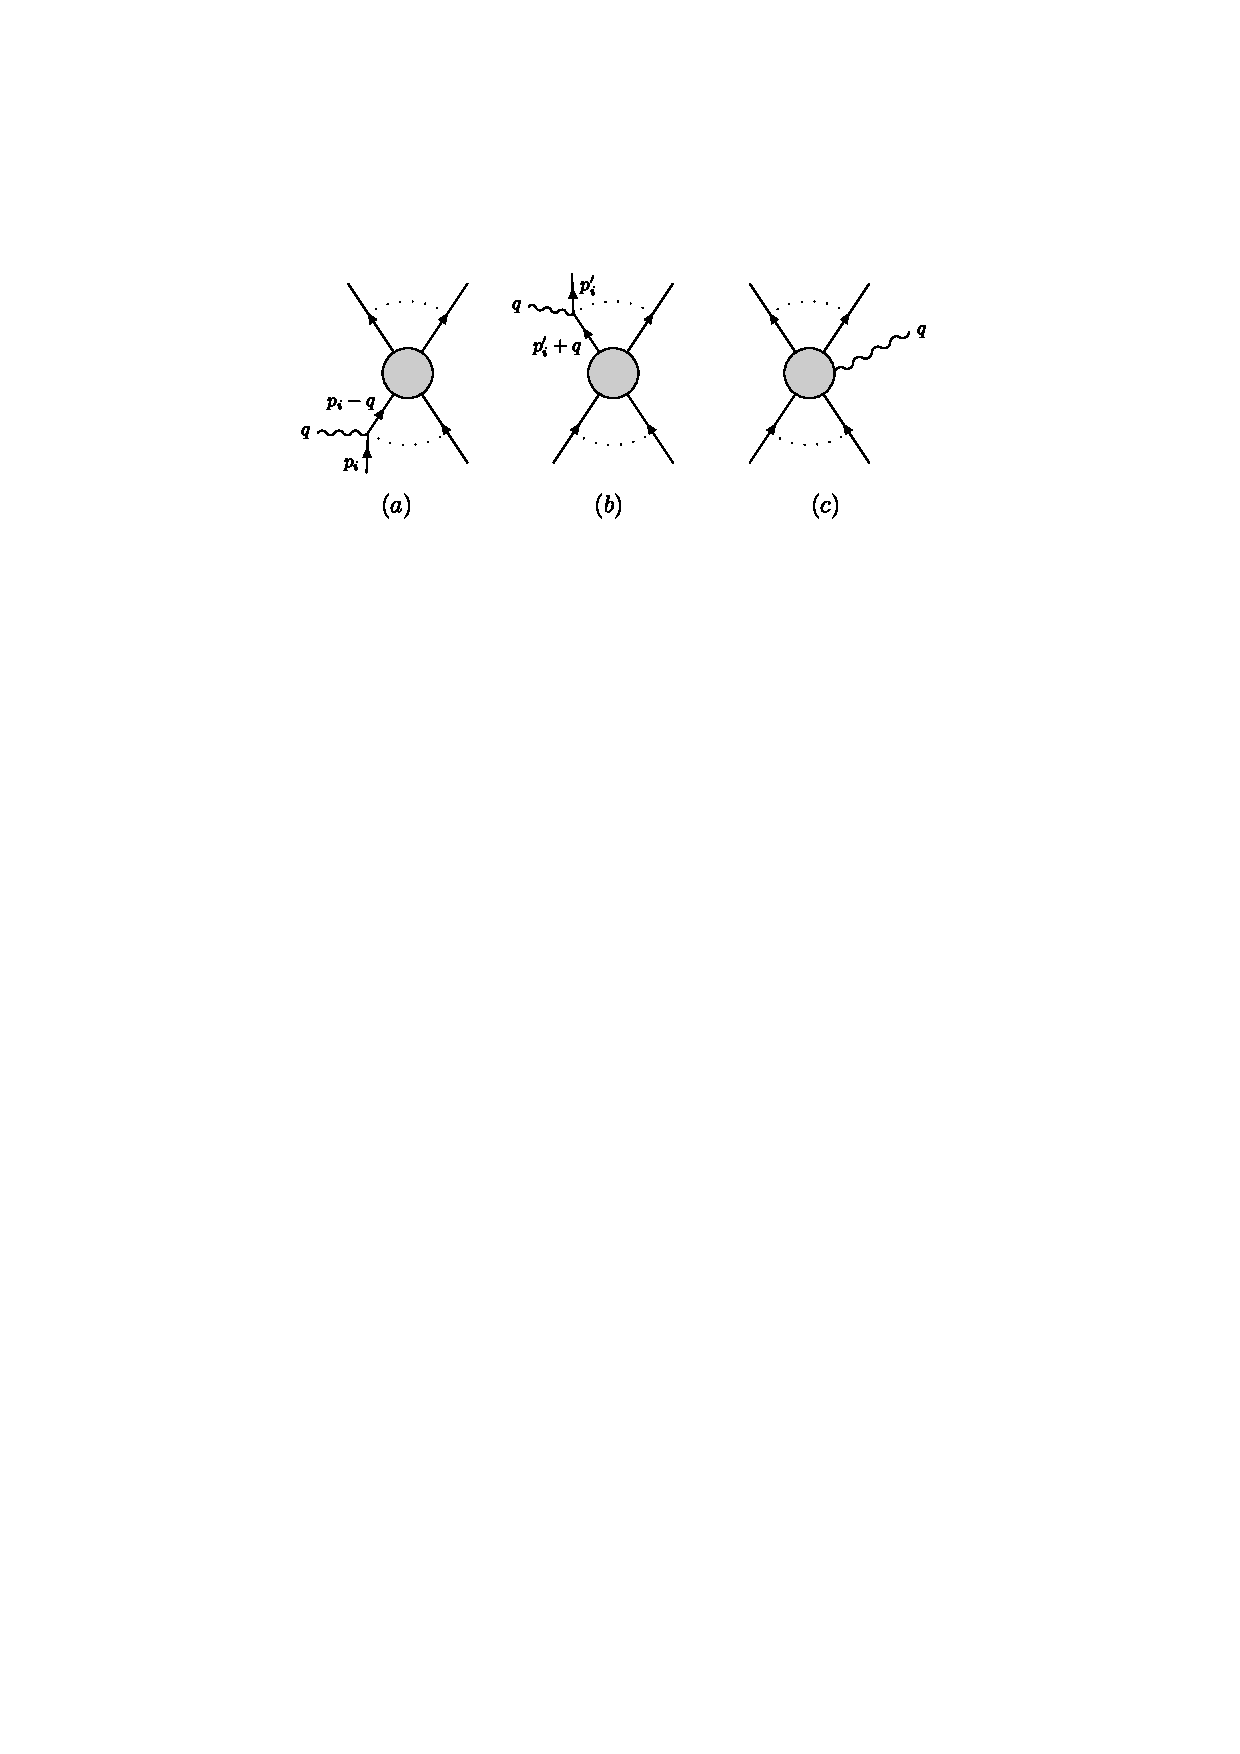
\includegraphics[width=0.8\linewidth]{figs/fig3.pdf}
	\caption{辐射软光子的三种情况}
\end{figure}
我们使用$\mathcal{A}(p,q)$表示辐射一个软光子后的振幅$\mathcal{A}(p)$表示没有辐射软光子的振幅(所有阶费曼图求和)。用$T(p_i-q)$表示原先没有辐射软光子的费曼图砍掉一个$p_i$外线但保留外线动量为非在壳的$p_i-q$得到的费曼图振幅,显然$T(p_i)u(p_i)=\mathcal{A}(p)$。

首先计算入射外线辐射软光子:
\begin{equation}
	\begin{aligned}
		Q_iT(p_i-q)\frac{(-\slashed{p}_i^\prime+\slashed{q}+m)\slashed{\epsilon}(q)}{(p_i-q)^2+m^2}u(p_i)&=-Q_iT(p_i-q)\Big[\frac{\epsilon(q)\cdot p_i+i\epsilon(q)_\mu q_\nu S^{\mu\nu}}{q\cdot p_i+\mathrm{i}0^+}\Big]u(p_i)
	\end{aligned}
\end{equation}
其中利用了$\slashed{a}\slashed{b}=-2a\cdot b-\slashed{b}\slashed{a}$,$q\cdot \epsilon_\pm(q)=0$以及狄拉克方程$(\slashed{p}+m)u(p)=0$。其中$S^{\mu\nu}=\frac{\mathrm{i}}{4}[\gamma^\mu,\gamma^\nu]$。唯一做近似的地方就是分母里面的$q^2$我们略去了,这对后面的高阶修正也不会影响。这一注意到$q=0$实际上是一个极点,这是因为在光子无线“软”的时候,多出来的那条内线传播子会无线趋于在壳,导致分母为0。

对于出射粒子辐射软光子也是类似的计算得到:
\begin{equation}\label{eq:20.17}
	\begin{aligned}
		Q^\prime_i\bar u(p_i^\prime)\frac{(-\slashed{p}_i^\prime-\slashed{q}+m)\slashed{\epsilon}(q)}{(p_i-q)^2+m^2}\bar T(p_i+q)&=-Q^\prime_i\bar u(p_i^\prime)\Big[\frac{\epsilon(q)\cdot p_i-i\epsilon(q)_\mu q_\nu S^{\mu\nu}}{q\cdot p_i-\mathrm{i}0^+}\Big]\bar T(p_i-q)
	\end{aligned}
\end{equation}

至于内线发射光子,我们用$N^\mu(p,q)$表示,而且注意到$q\to0$时$N\to0$,而且内线本身就是不在壳的,所以可以认为$N^\mu(p,q)\sim\mathcal{O}(q)$。三项加起来得到:
\begin{equation}
	\begin{aligned}
		\mathcal{A}(p,p^{\prime},q) =&\sum_\text{incoming }{ - Q _ i T ( p _ i - q )}\frac{\epsilon(q)\cdot p_i+i\epsilon(q)_{\mu}q_\nu S^{\mu\nu}}{q\cdot p_i+\mathrm{i}0^+}u(p_i)  \\
		&+\sum_{\mathrm{outgoing}}Q_{i}^{\prime}\bar{u}(p_{i}^{\prime})\frac{\epsilon(q)\cdot p_{i}^{\prime}-i\epsilon(q)_{\mu}q_{\nu}{S}^{\mu\nu}}{q\cdot p_{i}^{\prime}-\mathrm{i}0^+}\bar{T}(p_{i}^{\prime}+q)
		&+\epsilon(q)_{\mu}N^{\mu}(p,p^{\prime},q)
	\end{aligned}
\end{equation}
考虑最低阶修正,也就是只保留极点,得到:
\begin{equation}\label{eq:21.4}
	\boxed{
	\mathcal{A}(p,q)=\left[\sum_{i}\eta_iQ_{i}\frac{\epsilon(q)\cdot p_{i}}{q\cdot p_{i}}\right]\mathcal{A}(p)}+\mathcal{O}(1)
\end{equation}
其中对于入射粒子$\eta_i=-1$,出射粒子为$+1$。QED中辐射出光子的振幅都可以拆分成$\epsilon(q)_\mu \mathcal{M}^\mu$,振幅是相对论不变量,但是我们虽然常说$\epsilon(q)_\mu$是极化矢量,但它并不是真正意义上的矢量,因为其在lorentz变换下并不协变,而是会多出来一个正比于$q$的项\sn{我们是在Lorentz变换的意义下理解,其实矢量的这种变换完全可以理解为规范选取不同,从而从振幅的规范不变性导出结果。\cite{srednicki}}\cite{Weinberg}。为了让振幅是相对论不变量,必须有:
\begin{equation}\label{eq:21.5}
	\boxed{
	q_\mu\mathcal{M}^\mu=0}
\end{equation}
也就是Ward恒等式,也可以从Ward-高桥恒等式在U(1)对称性下导出它,实际上也就是利用电荷守恒导出它,但是前面我们的导出仅仅依赖于Lorentz不变性。现在把\ref{eq:21.4}中的$\epsilon(q)$替换为$q$我们得到:
\begin{equation}
	\left[\sum_i\eta_i Q_i\right]\mathcal{A}(p)=0
\end{equation}
也就是说,如果散射过程不被禁闭,也就是$\mathcal{A}(p)\neq 0$,那么这个过程必然要电荷守恒!另外说一句,我们这里的推导得到的\ref{eq:21.4}对于任意自旋的场都适用,比如对于标量QED,只需要把$S^{\mu\nu}$替换为0就好,不同的自旋对应$S^{\mu\nu}$的不同表示。

现在继续考虑两个光子的情况,两个光子由不同外线发射,在最低阶近似下只是乘上了\ref{eq:21.4}中两个因子,但是由相同外线发射就要考虑发射的先后顺序,因子形式会变化:
\begin{figure}[H]
	\centering
	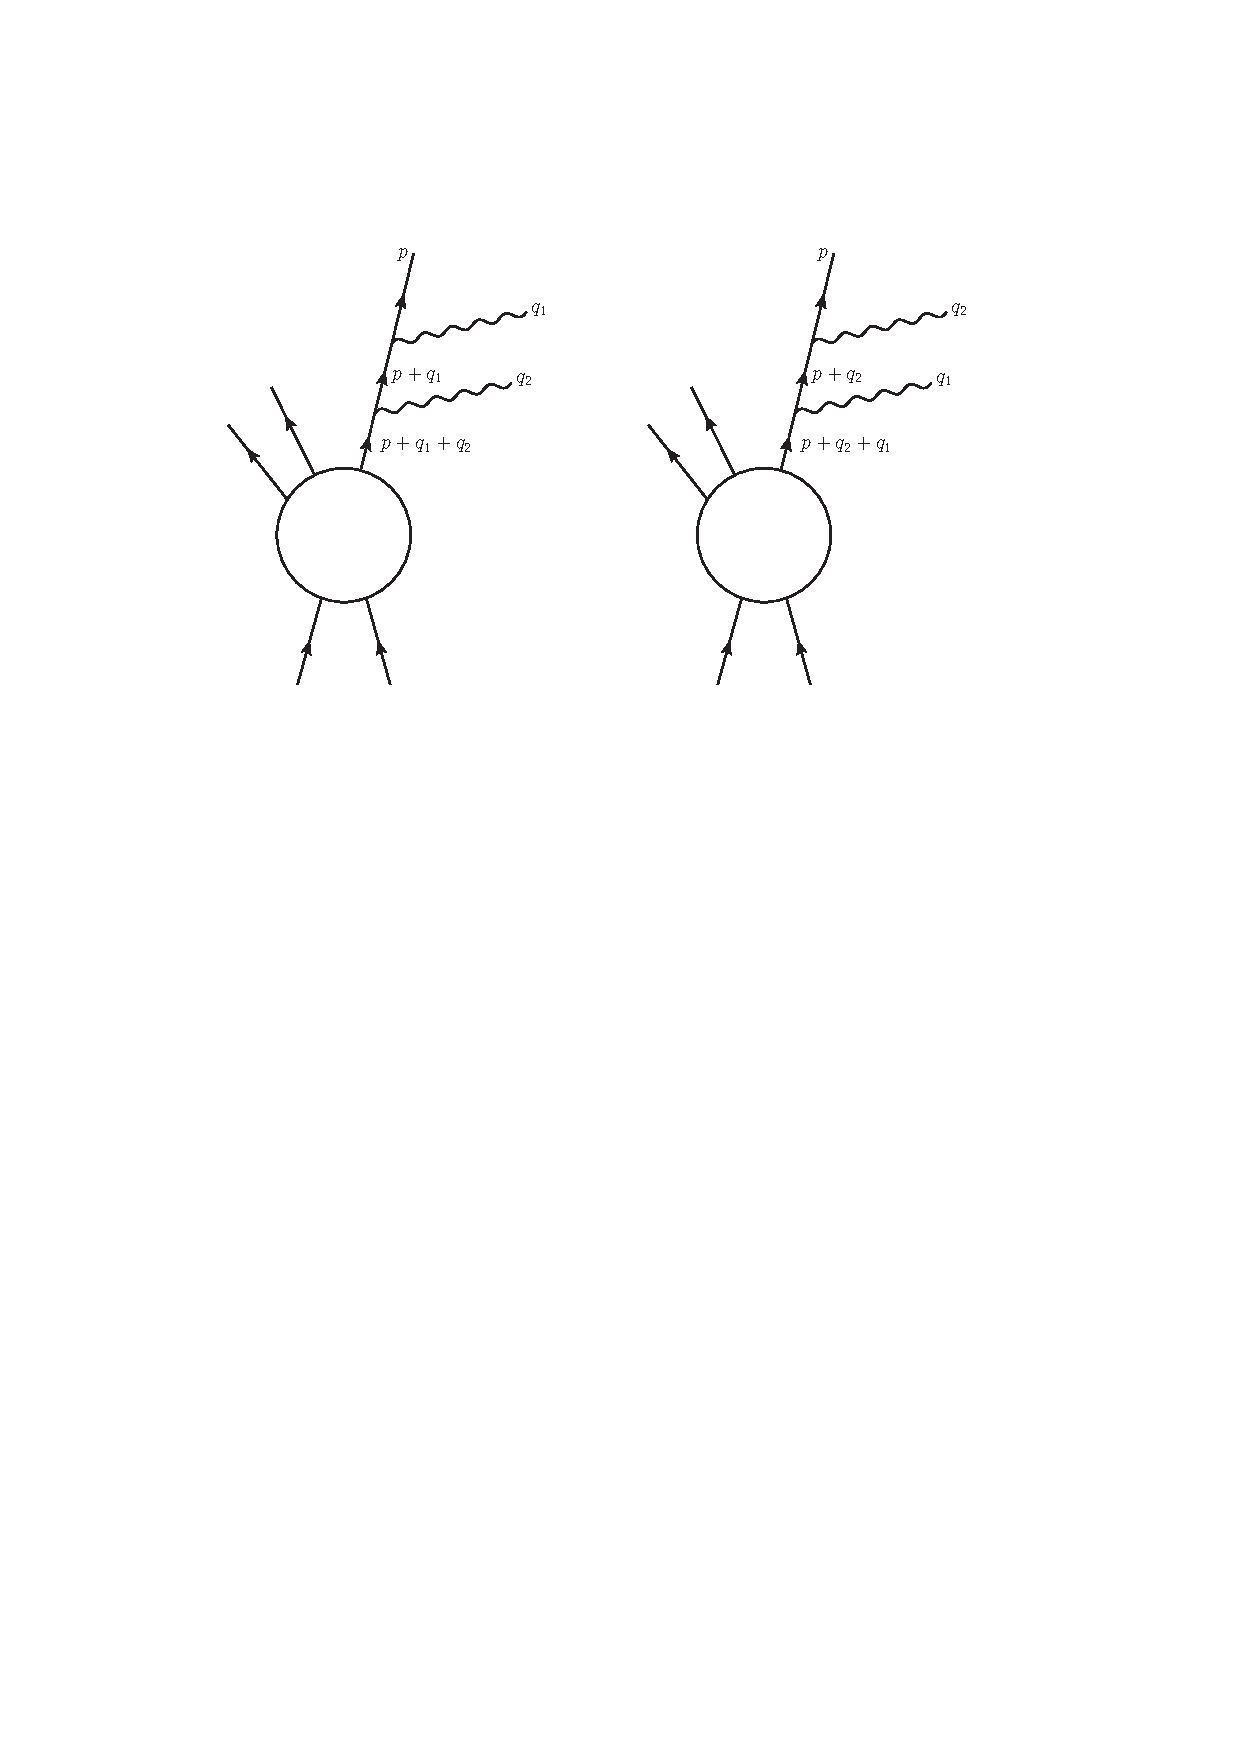
\includegraphics[width=0.8\linewidth]{figs/fig4.pdf}
	\caption{同一外线辐射两个软光子}
\end{figure}
把两幅图贡献的因子加起来得到:
\begin{equation}
	\begin{aligned}
	&\left[\frac{\eta Q\epsilon(q_1)\cdot p}{p\cdot q_1-\mathrm{i}\eta0^+}\right]\left[\frac{\eta Q\epsilon(q_2)\cdot p}{p\cdot(q_2+q_1)-\mathrm{i}\eta 0^+}\right]+\left[\frac{\eta Q\epsilon(q_2)\cdot p}{p\cdot q_2-\mathrm{i}\eta0^+}\right]\left[\frac{\eta Q\epsilon(q_1)\cdot p}{p\cdot(q_1+q_2)-\mathrm{i}\eta 0^+}\right]\\=&\left[\frac{\eta Q\epsilon(q_1)\cdot p}{p\cdot q_1-\mathrm{i}\eta0^+}\right]\left[\frac{\eta Q\epsilon(q_2)\cdot p}{p\cdot q_2-\mathrm{i}\eta 0^+}\right]	
	\end{aligned}
\end{equation}
得到的结果就是不同外腿上面的辐射两个软光子得到的因子,利用数学归纳法可以证明这一结论对于辐射任意数量的软光子都是适用的,那么最终我们只需要把因子乘起来,然后对所有外腿求和就好了,用式子表示如下:
\begin{equation}
	\boxed{\mathcal{A}(p,q_1,\ldots,q_m)=\prod_{j=1}^m\left[\sum_{i=1}^nQ_i\eta_i\frac{\epsilon(q_j)\cdot p_i}{q_j\cdot p_i}\right]\mathcal{A}(p)++\mathcal{O}(1)}
\end{equation}
前面的因子称为\textbf{eikonal因子}。推广到non-Abelian Y-M场的软定理也早有人计算过了\cite{Berends:1987me,Berends:1988zn,Mangano:1987kp,Mangano:1990by},软定理更多更一般的推广见\cite{McLoughlin:2022ljp}的文献索引。

现在来考虑辐射一个软引力子的情况,考虑第一节引入的标量场模型,传播子为:
\begin{equation}
	-\frac{i }{(p+\eta q)^2+m^2}
\end{equation}
顶点由\ref{eq:20.17}给出,但是由于\ref{eq:20.10},要与$\epsilon^{\mu\nu}$缩并,正比于$\eta_{\mu\nu}$的项没有贡献。以出射外线辐射软引力子为例,给出因子:
\begin{equation}
	i\sqrt{32\pi G}\varepsilon^{\mu\nu}p_{\mu}p_{\nu}\frac{-i}{\left(p+q\right)^{2}+m^{2}}\rightarrow\sqrt{8\pi G}\frac{\varepsilon^{\mu\nu}p_{\mu}p_{\nu}}{p\cdot q}
\end{equation}
求和后得到:
\begin{equation}
	\boxed{
	\mathcal{A}(p,q)=\left[\sum_i\frac{\kappa_i}{2}\eta_i\frac{\epsilon_{\mu\nu}(q)p_i^\mu p_i^\nu}{q\cdot p_i}\right]\mathcal{A}(p)+\mathcal{O}(1)}
\end{equation}

引力子同样有类似于\ref{eq:21.5}的恒等式,由此我们可以得到所有的$\kappa_i$都是相等的\sn{这里有点循环论证了,因为前面为了推导的方便我们同一取$\kappa_i=\sqrt{32\pi G}$},也就是等效原理!而自旋大于二的软粒子的软定理沿用上面的方法给出的限制就太强了,以至于散射$\mathcal{S}$矩阵必须trivial,所以一般认为自旋大于二的无质量粒子在“变软”的时候就脱耦合了。
\section{Subleading and subsubleading order soft theorem}

\section{Massless QED}
本章用天球的视角来看QED理论,为下一节做准备,本节的讨论都局限于比较简单的,不含磁荷而且电子没有质量的QED理论,但是基于此推出的许多结论实际上是普适的,可以推广到有质量QED上\cite{Strominger:2017zoo}。

弯曲时空中QED作用量:
\begin{equation}
	S_{EM}=-\frac{1}{2e^2}\int{F}\wedge\star F +S_M=-\frac{1}{4e^2}\int \mathrm{d}^4x\sqrt{-g}F_{\mu]nu}F^{\mu\nu}+S_M
\end{equation}
其中$S_M$由$j^\nu A_\nu$形式给出相互作用项,即$j^\nu=-\frac{\delta S_M}{\delta A^\nu}$。Maxwell场方程有下面简洁形式:
\begin{equation}
	\begin{cases}
		dF=0&\Rightarrow \nabla_\mu F_{\nu\rho}+\nabla_\nu F_{\rho\mu}+\nabla_\rho F_{\mu\nu}=0\\
		d\star F=e^2\star j&\Rightarrow \nabla_\mu F_{\mu\nu}=e^2j_\nu
	\end{cases}
\end{equation}
下式给出了整个空间内的净电荷/磁荷\sn{后文$\star,*$指的都是Hodge dual}:
\begin{equation}
	Q_E=\frac{1}{e^2}\int_{\mathcal{S}^2_\infty}\star F=\int_{\Sigma}\star j,\quad Q_M=\frac{1}{2\pi}\int_{\mathcal{S}^2_\infty} F
\end{equation}
它们是量子化的,只能取整数。QED是$U(1)$规范理论,在$A\mapsto A+d\varepsilon$的规范变换下理论不变,后文不加说明都在所谓\textbf{retarded radial 规范}下进行计算\cite{Lee:1990nz}:
\begin{equation}
	\begin{aligned}
		&\mathcal{I}^+: A_r=0,\quad A_u|_{\mathcal{I}^+}=0\\
		&\mathcal{I}^-: A_r=0,\quad A_v|_{\mathcal{I}^-}=0
	\end{aligned}
\end{equation}
在$\mathcal{I}^{\pm}$附近可以把$A,F$展开成$\mathcal{O}(1/r)$的形式,用$A^{(i)},F^{(i)}$表示$r^{-i}$项前的系数,那么在这一规范下有:
\begin{equation}
	F_{ur}^{(0)}=A_u^{(0)}=0, F_{z\bar z}^{(0)}=\partial_z A_{\bar z}^{(0)}-\partial_{\bar z}A_z^{(0)},F_{uz}^{(0)}=\partial_u A_z^{(0)},F_{rz}^{(0)}=-A_z^{(1)}
\end{equation}
$\mathcal{I}^-$处类似。但这个规范选取就如库伦规范$\nabla\cdot \mathbf{A}=0$一样没有完全确定规范,$A_z$还可以进行下面的所谓Large gauge transformation:
\begin{equation}
	A_z\mapsto A_z+\partial_z\varepsilon(z,\bar z),\quad \forall \varepsilon\in C^\infty\left[C\mathcal{S}^2\right]
\end{equation}
运动电荷激发的电磁场即所谓Li\'enard\mbox{-}Wiecher势\cite{Jackson1998ClassicalE3}。这里我们在天球坐标下将advanced和retarded势统一写为:
\begin{equation}
	F_{rt}(\vec{x},t)=\frac{e^2}{4\pi}\sum_{k=1}^n\frac{Q_k\gamma_k\left(r-t\hat{x}\cdot\vec{\beta}_k\right)}{\left|\gamma_k^2\left(t-r\hat{x}\cdot\vec{\beta}_k\right)^2-t^2+r^2\right|^{3/2}},\quad r^2=\vec{x}\cdot\vec{x},\quad\vec{x}=r\hat{x}
\end{equation}
其中我们假设所有电荷之间匀速运动,而且相互作用可忽略,这个假设有点强,但是请\textbf{相信}后面导出的结论是可以推广到一般情形的。现在计算在天球上的极限:
\begin{equation}
	\begin{aligned}
		&\left.F_{rt}\right|_{\mathcal{I}^{+}}=\frac{e^{2}}{4\pi r^{2}}\sum_{k=1}^{n}\frac{Q_{k}}{\gamma_{k}^{2}(1-\hat{x}\cdot\vec{\beta}_{k})^{2}}\\
		&\left.F_{rt}\right|_{\mathcal{I}^{-}}=\frac{e^{2}}{4\pi r^{2}}\sum_{k=1}^{n}\frac{Q_{k}}{\gamma_{k}^{2}(1+\hat{x}\cdot\vec{\beta_{k}})^{2}}
	\end{aligned}
\end{equation}
取极限,得到:
\begin{equation}
	\boxed{
	\left.F_{rt}\right|_{\mathcal{I}^{+}_-}\neq \left.F_{rt}\right|_{\mathcal{I}^{-}_+}}
\end{equation}
正是这个式子说明了要严格区分$\mathcal{I}^{+}_-,\mathcal{I}^{-}_{+}$和$i^0$。但是,因为$F_{ru}=F_{rt}=F_{rv}$:
\begin{equation}
	\boxed{
		\lim\limits_{r\to\infty}r^2F_{ru}(\hat{x})\Big|_{\mathcal{I}_{-}^+}=\lim\limits_{r\to\infty}r^2F_{rv}(-\hat{x})\Big|_{\mathcal{I}_{+}^-}
	}
\end{equation}
也就是说场在两个天球上是对径认同的,这也是为什么前面$\mathcal{I}^{\pm}$天球的角向选取是antipodal的,上边的式子可以写成下面很简洁的形式:
\begin{equation}
	\boxed{
	\left.F_{ru}^{(2)}(z,\bar z)\right|_{\mathcal{I}^{+}_-}=\left.F_{rv}^{(2)}(z,\bar z)\right|_{\mathcal{I}^{-}_+}
	}
\end{equation}
这个式子是普适的,而且非常重要,是后面散射问题的核心。现在考虑任意一个天球上的对径认同的函数:
\begin{equation}
	\varepsilon(z,\overline{z})|_{\mathcal{I}_{-}^{+}}=\varepsilon(z,\overline{z})|_{\mathcal{I}_{+}^{-}}
\end{equation}
定义下面的future charges和past charges:
\begin{equation}
	\boxed{
		Q_{\varepsilon}^{+}=\frac{1}{e^{2}}\int_{\mathcal I_{-}^{+}}\varepsilon*F,\quad Q_{\varepsilon}^{-}=\frac{1}{e^{2}}\int_{\mathcal I_{+}^{-}}\varepsilon*F
	}
\end{equation}
由于Hodge对偶后出来的体积元$\propto r^2$,所以在天球上$r\to\infty$,$F\to F^{(2)}$,再根据对径认同的条件,这样对于任意一个函数$\varepsilon$,我们都给出了一个“电荷”守恒律:
\begin{equation}
	\boxed{
	Q_\varepsilon^+=Q_\varepsilon^-
	}
\end{equation}
对于$\varepsilon$是常函数情形,就得到了一般的电荷守恒律。利用Stokes公式\sn{$\int_{\partial \Omega}\omega =\int_{ \Omega}d\omega$}可以改写$Q_\varepsilon^{\pm}$为\sn{$Q_\varepsilon^-$只用把$+\mapsto -$}:
\begin{equation}
	Q_\varepsilon^+=\frac{1}{e^2}\int_{\mathcal{I}^+}\mathrm{d}\varepsilon\wedge*F+\int_{\mathcal{I}^+}\varepsilon*j+\cancelto{0}{\frac{1}{e^2}\int_{\mathcal{I}_+^+}\varepsilon*F}
\end{equation}
最后一项为0是因为我们假设电子是无质量的,这样电子就是从$\mathcal{I}^-\to\mathcal{I}^+$,而不是$i^{-}\to i^+$,所以$F|_{\mathcal{I}_+^{+}}=0$。第一项是Soft term $Q_S^+$与软光子的产生湮灭有关,第二项由于是与流耦合,所以叫Hard term $Q_H^+$与带电实物粒子有关。将上面的微分形式写成分量形式\sn{其中使用了Bianchi恒等式:$\partial_{u}F_{ru}^{(2)}+D^{z}F_{uz}^{(0)}+D^{\bar{z}}F_{u\bar{z}}^{(0)}+e^2j_{u}^{(2)}=0$}:
\begin{equation}
	Q_{\varepsilon}^{+}=\underbrace{-\frac{1}{e^{2}}\int_{\mathcal{I}^{+}}dud^{2}z\left(\partial_{z}\varepsilon F_{u\bar{z}}^{(0)}+\partial_{\bar{z}}\varepsilon F_{uz}^{(0)}\right)}_{Q_{S}^{+}}+\underbrace{\int_{\mathcal{I}^{+}}dud^{2}z\varepsilon\gamma_{z\bar{z}}j_{u}^{(2)}}_{Q_{H}^{+}}
\end{equation}
\section{Ward indentity = Soft theorem}